\chapter{Forschungsstand und verwandte Arbeiten}

In diesem Abschnitt werden die aktuellen Forschungsstände von Technologien beschrieben, die für das Verständnis und die Umsetzung des Projekts wesentlich sind. Dazu gehören der aktuelle Stand der Textzusammenfassung, \ac{LLM}s, LaTeX, \ac{DOCX} und Web-Entwicklung.

\section{Forschungsstand}
\begin{description}
    \item[Die Textzusammenfassung] per Hand erweist sich als sehr mühsam, da die Masse an Texten im Internet stetig steigt. Aus diesem Grund wird versucht, die Textzusammenfassung zu automatisieren. Dabei wurde eine Formel aufgestellt, die die Kompressionsrate $\tau$ des Textes berechnet. \cite[S.1]{yadav2022automatictextsummarizationmethods}

    \begin{align}
    \mathlarger{\tau = \frac{| \text{Summary} |}{| \text{Source} |}}
    \end{align}

    Es wurde festgestellt, dass bei einer generierten Zusammenfassung die beste Leistung bei einer Kompressionsrate von 15-30\% erzielt wird \cite[S.1]{yadav2022automatictextsummarizationmethods}. Bei einer Kompressionsrate von weniger als 15\% kann es vorkommen, dass für die Verständlichkeit wichtige Informationen fehlen. Der Text wird kompakt, aber möglicherweise unvollständig, und der Kontext geht verloren. Umgekehrt werden bei einer Kompressionsrate von mehr als 30\% zu viele Details beibehalten, was dazu führt, dass die Funktion einer kurzen und prägnanten Zusammenfassung nicht mehr erfüllt wird.

    Eine Zusammenfassung kann auf zwei Arten erfolgen, die in der Abbildung \ref{fig:Extractive text summarizer and Abstractive text summarizer} dargestellt sind. Die Extraktive Textzusammenfassung entnimmt Sätze aus dem originalen Textkorpus und setzt diese in der Zusammenfassung zusammen. Die Abstrake Zusammenfassung hingegen erstellt aus dem originalen Text neue Sätze und bildet dadurch die Zusammenfassung. \cite[S.3]{yadav2022automatictextsummarizationmethods}

    \begin{figure}[H]
    \centering
    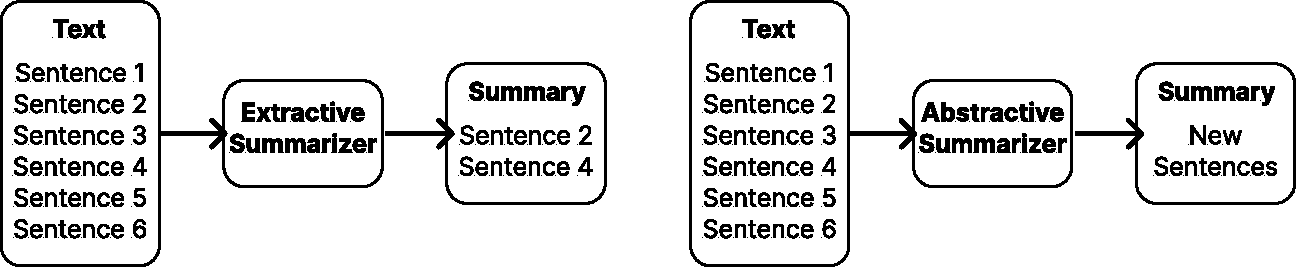
\includegraphics[width=0.8\linewidth]{Images/Extractive text summarizer and Abstractive text summarizer.pdf}\\
    \caption{Extractive and Abstractive text summarizer \cite[S.3]{yadav2022automatictextsummarizationmethods}}
    \label{fig:Extractive text summarizer and Abstractive text summarizer}
    \end{figure}

    
    \item[Die \ac{LLM}s] stehen durch das Wachstum des Internets große Informationsmengen zur Verfügung. Sie können kurze Zusammenfassungen von Quelltexten erstellen, ohne den Gesamtzusammenhang zu verlieren. Allerdings muss man bei der Verwendung von \ac{LLM}s vorsichtig sein und den Output kontrollieren, da zum Beispiel Halluzinationen auftreten können. Unter Halluzinationen versteht man Ausgaberesultate von \ac{LLM}s, die weder real noch im gelernten Datensatz enthalten sind. \cite[S.1]{banerjee2023benchmarkingllmpoweredchatbots}

    In Fisher's \ac{LLM} Comparison Research zeigt sich, dass \ac{LLM}s eine Möglichkeit bieten, Zeit zu sparen. Dennoch ist es notwendig, dass jemand die generierten Daten überprüft \cite{fisher2024large}. Es zeigt sich auch, dass \ac{LLM}s noch nicht an von Menschen geschriebene Texte heranreichen. Denn die von \ac{LLM}s generierten Texte sind umfangreich, folgen einer logischen Struktur und wiederholen sich häufig. Im Gegensatz dazu ist menschliches Schreiben vielfältig und unterschiedlich, da jeder Mensch eine andere Art hat, sich auszudrücken. Es wurde jedoch festgestellt, dass sich \ac{LLM}s ebenso wie menschliche Autoren voneinander unterscheiden \cite{rosenfeld2024whose}. Es bleibt abzuwarten, ob \ac{LLM}s in Zukunft so sprachgewandt werden wie Menschen.

     Ein weiterer interessanter Aspekt im Zusammenhang mit der Entwicklung von Prompts für \ac{LLM}s ist der von Levi und Neumann getestete Jailbreak-Angriff. Diese Attacke zielt darauf ab, den Sicherheitsmechanismus eines Sprachmodells zu umgehen. Dabei werden gezielt unauffällige Wörter oder Trennzeichen in Prompts eingefügt, um unerwünschte oder gefährliche Antworten zu provozieren. Selbst scheinbar harmlose Veränderungen des Prompts können das Verhalten des Modells erheblich beeinflussen \cite{levi2024vocabularyattackhijacklarge}. Die Sicherheit von \ac{LLM}s spielt daher heute eine zentrale Rolle, insbesondere bei der Entwicklung von Modellen für die breite Öffentlichkeit.
    
    \item[LaTeX] ist ein Textsatzsystem, das vor allem in wissenschaftlichen Kreisen zur Erstellung von Dokumenten verwendet wird. Es bietet erweiterte Funktionen für die Darstellung komplexer mathematischer Formeln und Referenzierungen. Die Verwendung von LaTeX ermöglicht eine präzise Kontrolle über das Layout und die Formatierung, was besonders bei umfangreichen Dokumenten von Vorteil ist.

    Aktuelle Entwicklungen in LaTeX zielen darauf ab, die Zugänglichkeit und Wiederverwendbarkeit eines \ac{PDF} zu verbessern, um Standards wie \ac{PDF}/\ac{UA} zu erfüllen. Diese Entwicklungen sind bereits seit einigen Jahren im Gange und 2024 wurde ein Prototyp erstellt, der diesen Standards entspricht.  \cite{mittelbach2024accessible}
    
    \item[\ac{DOCX}] ist eines der am weitesten verbreiteten Formate zur Erstellung und Bearbeitung von Textdokumenten. Es bietet eine breite Palette an Funktionen für Textformatierung, Multimedia-Integration und Layoutgestaltung.
    
    Eine der neuesten Funktionen von \ac{DOCX} ist die Integration von Copilot. Copilot ist eine \ac{KI}, die Benutzer beim Entwerfen und Schreiben von Dokumenten unterstützt. Sie bietet Möglichkeiten, Texte in Tabellen umzuwandeln, Texte umzuschreiben und mit dem Benutzer in einem interaktiven Chat zu kommunizieren. Zudem kann Copilot auch Zusammenfassungen generieren, was den Schreibprozess erleichtert. \cite{microsoft_copilot}
    
    \item[Die Web-Entwicklung]hat in den letzten Jahren bedeutende Fortschritte gemacht und ist zu einem der zentralen Bereiche der Informatik geworden. Insbesondere die Frontend-Entwicklung mit JavaScript-Frameworks wie React, Angular und Vue.js wird immer beliebter. Die Analyse von Vyas zeigt, dass React mit 35,9\% der Entwickler derzeit das beliebteste Framework ist. Außerdem zeigt Vyas mit Hilfe von Google Trends, dass React ein stabiles Wachstum aufweist, während Angular leicht rückläufig ist und Vue nur langsam wächst. \cite{vyas2022comparative} 
    
\end{description}

\section{Verwandte Webanwendungen}
In diesem Abschnitt werden verwandte Webanwendungen vorgestellt, welche ähnlich wie \textit{Reforge} mit \ac{KI} arbeiten und ebenfalls Zusammenfassungen generieren können. Sucht man im Browser nach Summary-Generatoren, so stößt man auf unzählige Seiten und Tools, die Texte zusammenfassen. Eine Handvoll dieser Tools wird näher betrachtet. Anschließend werden die Unterschiede des vorliegenden Projekts erläutert.

\begin{description}
    \item[Chat\ac{GPT}] ist ein \ac{KI}-basiertes Sprachmodell von OpenAI, das entwickelt wurde, um auf natürliche Weise mit Benutzern zu interagieren. Es ermöglicht beispielsweise das Schreiben von Texten, das Erlernen neuer Konzepte und das Sammeln von Ideen. In der mobilen Anwendung kann der Benutzer sogar eine Sprachkonversation starten. Außerdem können Antworten mit Links zu relevanten Webquellen abgerufen werden. Darüber hinaus bietet Chat\ac{GPT} die Möglichkeit, Dateien hochzuladen, um sie zu analysieren oder zusammenzufassen. Chat\ac{GPT} verfügt also über eine Vielzahl von Funktionen. \cite{openai_overview}

    \item[Microsoft Copilot] ist ein von Microsoft entwickelter \ac{KI}-Assistent, der sogar in Microsoft 365-Anwendungen integriert ist. Mit Hilfe von generativer \ac{KI} kann Copilot Inhalte erstellen und Daten analysieren. Er bietet auch eine Chat-Funktion, über die Nutzer Anweisungen an Copilot übermitteln können. \cite{microsoft_copilot_overview}

    \item[Google Gemini] ist eine von Google entworfene Chat-Anwendung mit künstlicher Intelligenz. Es hilft Nutzern bei Aufgaben wie Schreiben, Planen und Lernen. Durch die Eingabe von Textbefehlen können Nutzer direkt mit der \ac{KI} interagieren und erhalten passende Antworten. Gemini nutzt Informationen aus verschiedenen Quellen, einschließlich anderer Google-Dienste, um hilfreiche Antworten zu liefern. \cite{Gemini_overview}

    \item[Quillbot] ist ein \ac{KI}-gestütztes Schreibwerkzeug, das als Chrome-Erweiterung verfügbar ist. Es unterstützt den Benutzer bei der Verbesserung von Texten durch Funktionen wie Paraphrasierung, Grammatikprüfung und Tonerkennung. Darüber hinaus bietet es weitere Funktionen wie die Erstellung von Zusammenfassungen\footnote[1]{Quillbot: \href{https://quillbot.com/summarize}{https://quillbot.com/summarize}}. Außerdem bietet die Erweiterung sowohl kostenlose als auch kostenpflichtige Funktionen, um den unterschiedlichen Bedürfnissen der Nutzer gerecht zu werden.
    
\end{description}

\subsubsection{Unterscheidungsmerkmale von \textit{Reforge}}

Zusammenfassend unterscheidet sich das vorliegende Projekt von den genannten Lösungen durch folgende Eigenschaften:

\begin{itemize}
    \item \textit{Reforge} bietet keine Chat-Funktion, sondern nur Parameterfelder, die ausgefüllt werden müssen. Nach der Eingabe wird die Verarbeitung der Eingaben ähnlich wie bei Quillbot über einen Button gestartet.
    \item Ein wesentlicher Unterschied besteht in der Ausgabe. Der Nutzer kann wählen, ob er die Ausgabe als IEEEtran oder als OTH-Forschungsbericht erhalten möchte. Außerdem kann entschieden werden, ob der Technische Bericht in deutscher oder englischer Sprache erhalten werden soll. Diese Ausgabeparameter sind bei den genannten Werkzeugen nicht vorhanden.
    \item Das System bietet eine automatisierte Zusammenfassung von LaTeX-ZIP-Archive und \ac{DOCX}-Dokumenten mit Hilfe von \ac{LLM}s. Der Benutzer muss nicht wie bei ChatGPT oder Copilot Prompts an den \ac{LLM} senden.
\end{itemize}

Dieses Projekt stellt somit eine innovative Lösung zur Generierung von technischen Berichten aus LaTeX- oder \ac{DOCX}-Dokumenten dar. Der Benutzer ist flexibel und kann die gewünschte Ausgabe anpassen.